\documentclass[11pt]{article}
\newcommand{\numpy}{{\tt numpy}}    % tt font for numpy
\usepackage[margin=1in]{geometry}
\usepackage{graphicx}

\begin{document}

$$\mbox{\Large \textbf {CS 111 (S19): Homework 3}}$$
$$\mbox{\textbf {Due by 6:00pm Monday, April 22}}$$
$$\mbox{\textbf {NAME and PERM ID No.:} Chen Li, 5468137 (replace with yours)}$$
$$\mbox{\textbf {UCSB EMAIL:} chenli@ucsb.edu (replace with yours)}$$

\par\bigskip
{\bf 1.}
How many arithmetic operations 
(total of additions, subtractions, multiplications, divisions)
are required to do each of the following?
(You can omit lower-order terms in $n$.)

\par\medskip
{\bf 1a.} Compute the sum of two $n$-vectors?
$$n$$
\par\medskip
{\bf 1b.} Compute the product of an $n$-by-$n$ matrix with an $n$-vector?
$$n*(n+(n-1))=2n^2-n$$
\par\medskip
{\bf 1c.} Compute the product of two $n$-by-$n$ matrices?
$$n^2(n+(n-1))=2n^3-n^2$$
\par\medskip
{\bf 1d.} Solve an $n$-by-$n$ upper triangular linear system $Ux=y$?
$$2\sum_{i=1}^{n-1}i+n=(n-1)n+n=n^2
$$
\newpage

\par\bigskip
{\bf 2.}
Suppose $A$ and $B$ are $n$-by-$n$ matrices, with $A$ nonsingular,
and $c$ is an $n$-vector.
Describe the steps you would use to {\em efficiently} compute the
product $A^{-1}Bc$.
Describe a different, less efficient, sequence of steps.
\newline\newline Efficient: realizing that $AA^{-1}Bc = Bc$, then $A^{-1}Bc$ is the solution to $Ax = Bc$, so we can do gaussian elimination to solve x, which is the answer. In this way, we can avoid computing inverse, which take roughtly 3 time more steps than gaussian elimination when matrix is large.\newline\newline
Inefficient: inverse A, then calculate $A^{-1}Bc$, which take roughly 3 time more steps than previous one.
\newpage

\par\bigskip
{\bf 3.}
Suppose that $A$ is a square, nonsingular, nonsymmetric matrix, 
$b$ is an $n$-vector, and that you have called 
$$\mbox{\tt L, U, p = LUfactor(A)}$$
(using the routine from the lecture files).
Now suppose you want to solve the system $A^Tx=b$ (not $Ax=b$) for $x$.
Show how to do this using calls to {\tt Lsolve()} and {\tt Usolve()},
without modifying either of those routines or calling {\tt LUfactor()} again.
Test your method in {\tt numpy} on a randomly generated 6-by-6 matrix
(see {\tt np.random.rand()}).
\newline\newline Get Permutation matrix P from p\\
PA = LU\\
$A = P^TLU\\
A^T=U^TL^TP\\
A^Tx = U^TL^TPx =b$\\
let Px = y\\
$A^Tx = U^TL^Ty=b\\
$ therefore, $U^T$ is a lower triangle matrix and $L^T$ is a upper triangle matrix
\\then, $y = Usolve(L.T, Lsolve(U.T, b[p])$\\
and $x = P.Ty$\\
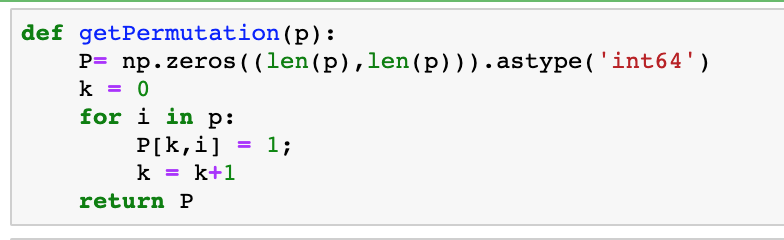
\includegraphics[scale=0.8]{534012.png}\\
here, lower p is permuting array, and upper P is permutation matrix that get returned\\
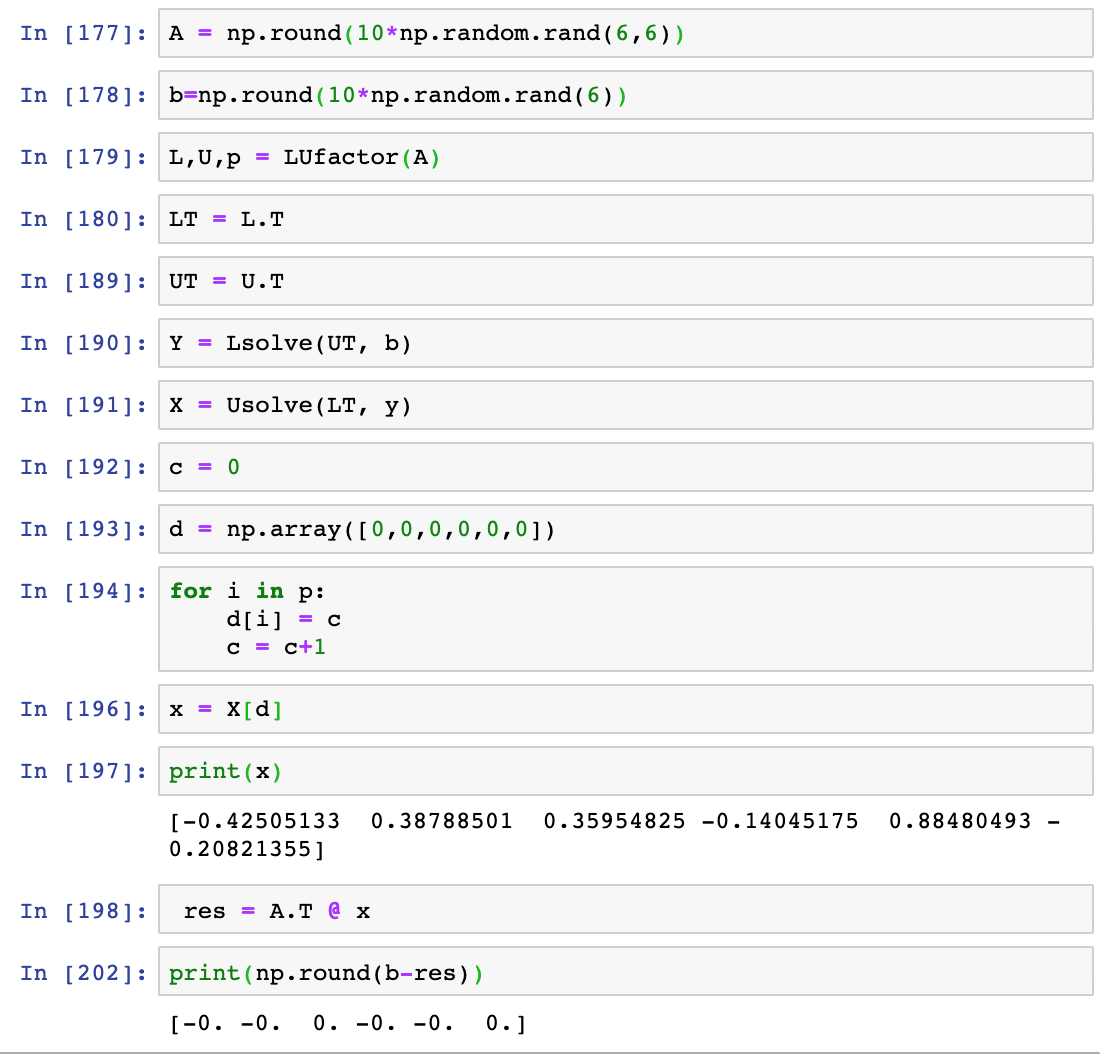
\includegraphics[scale=0.4]{kk.png}
\newpage

\par\bigskip
{\bf 4.} Do problem 2.3 on pages 32--33 of the NCM book, 
showing the {\tt numpy} code you use and its output. 
Note: To understand intuitively what the problem means by 
``assume that joint 1 is rigidly fixed both horizontally and vertically 
and that joint 8 is fixed vertically,'' 
think of the truss as a (2-dimensional) drawbridge across a river, 
with the left end being a hinge and the right end lying on the ground.\newline
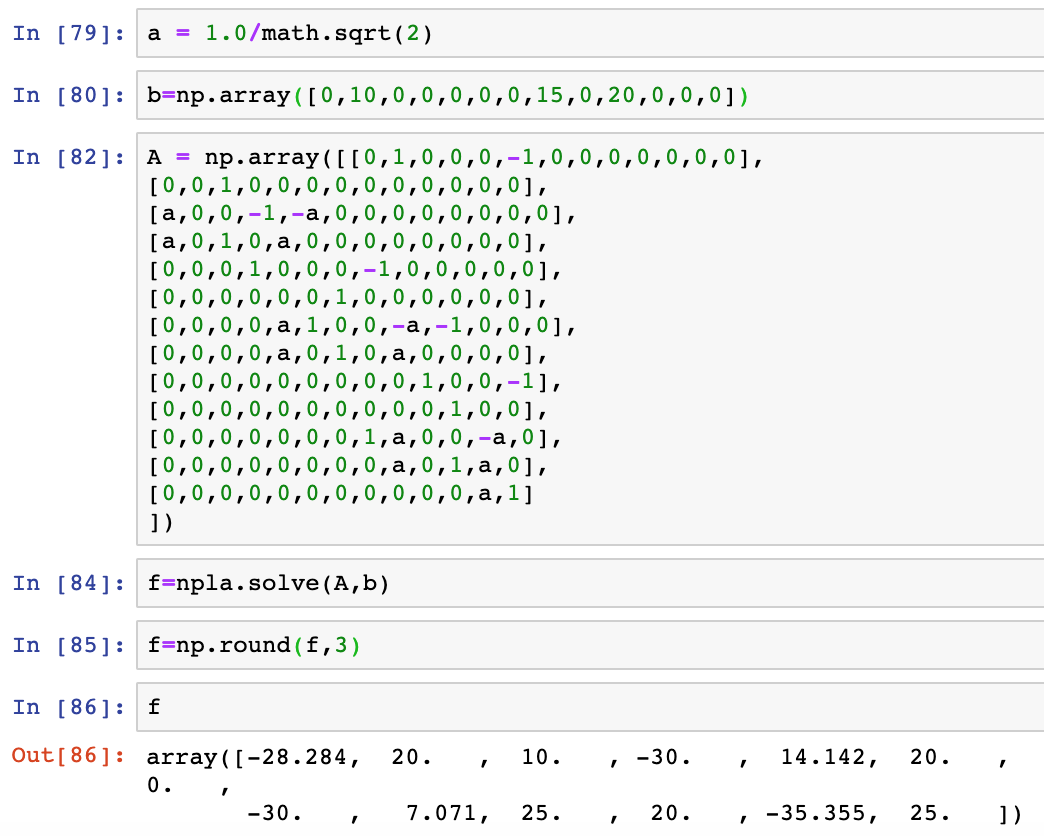
\includegraphics[scale=0.8]{P4H3}
%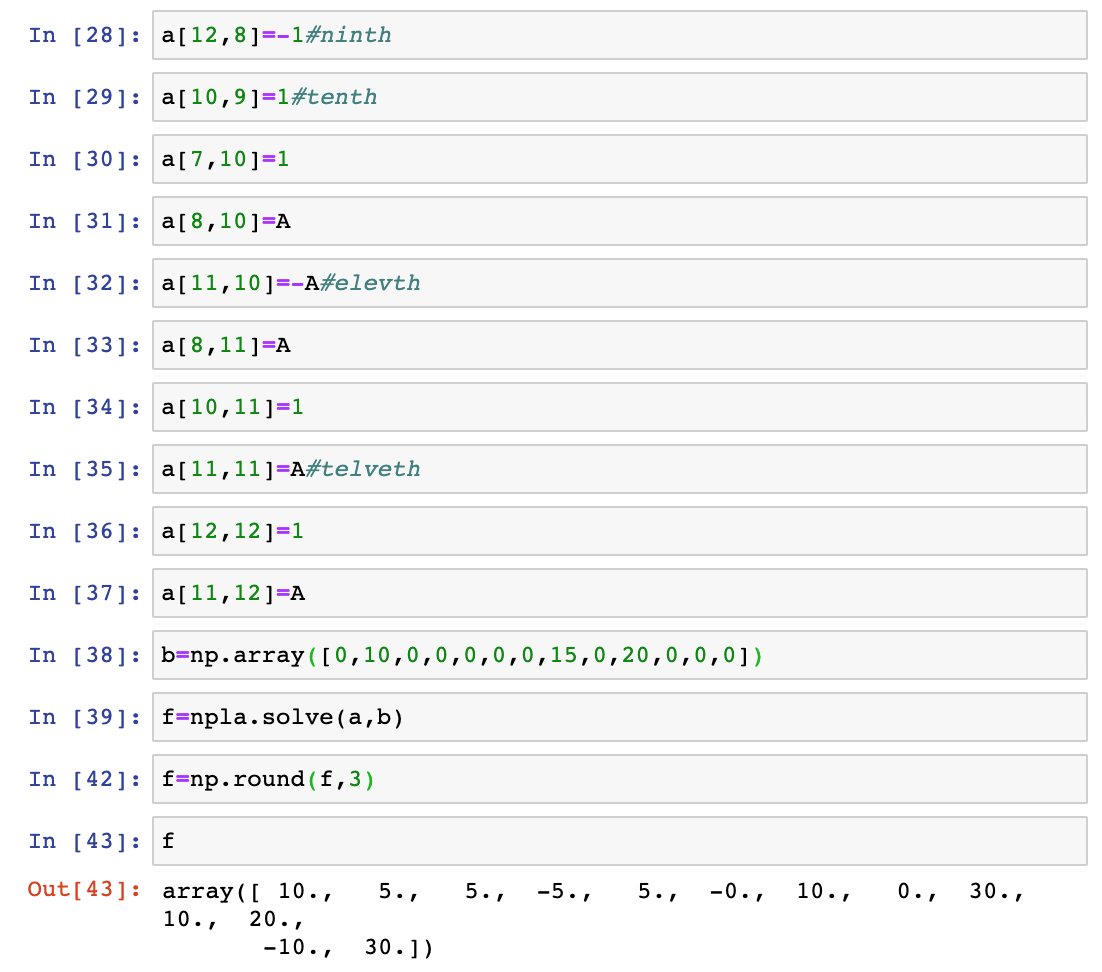
\includegraphics[scale=0.8]{pic2.png}
\newpage

\par\bigskip
{\bf 5.} Consider the linear system
$$
   \left(
   \begin{array}{cc}
      \alpha & 1 \\ 	
           1 & 1 \\ 	
   \end{array} \right)
   \left(
   \begin{array}{c}
      x_0 \\ 	
      x_1 \\ 	
   \end{array} \right)
   =
   \left(
   \begin{array}{cc}3
      \alpha + 2 \\ 	
               3 \\ 	
   \end{array} \right),
$$
for some $\alpha < 1$.
Clearly the solution is $(x_0, x_1)^T = (1,2)^T$.
For each value of $\alpha = 10^{-4}, 10^{-8}, 10^{-16}, 10^{-20}$,
solve this system using the routines {\tt LUfactor()}, {\tt Lsolve()}, 
and {\tt Usolve()} from {\tt LUsolve.ipynb} in the lecture files.
For each $\alpha$, do this twice, first with {\tt pivoting = True} in {\tt LUfactor()}
and then with {\tt pivoting = False}.
Show your {\tt numpy} code and its output.
Comment on your results.\newline
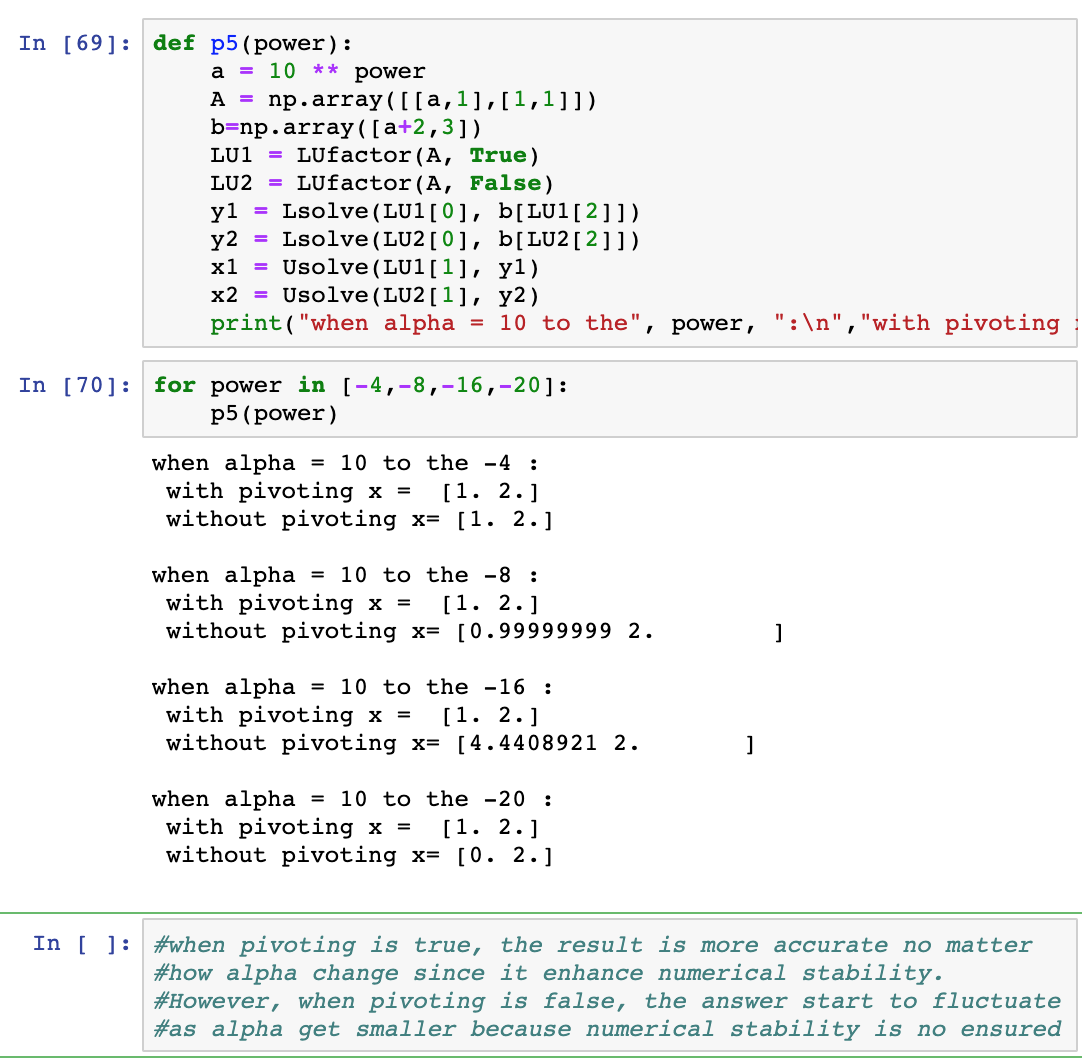
\includegraphics[scale=0.8]{p5.png}
\\by selete the pivot with maxium value in the column, we can enhanve stability
\newpage

\par\bigskip
{\bf 6.} Recall that a symmetric matrix $A$ is {\em positive definite}
(SPD for short) if and only if $x^TAx>0$ for every nonzero vector $x$.

\par\medskip
{\bf 6a.} Find a 2-by-2 matrix $A$ that (1) is symmetric, (2) is not singular,
and (3) has all its elements greater than zero, but (4) is {\em not} SPD.
Show a nonzero vector $x$ such that $x^TAx<0$.
$$A=\left(\begin{array}{cc}
	1&2\\
	2&1
\end{array}\right), x=(1,-1),\Rightarrow x^TAx=-2$$
\par\medskip
{\bf 6b.} Let $B$ be a nonsingular matrix, of any size, 
not necessarily symmetric.
Prove that the matrix $A=B^TB$ is SPD.\newline\newline
symmetric: $A^T=(B^TB)^T=B^T(B^T)^T=B^TB=A$\newline
positive definite: $x^TAx=x^TB^TBx=(Bx)^T(Bx)=y^Ty$, which is a inner product of a non-zero vector y (since B is nonsingular and x is non-zero), alway larger than 0.

\end{document}
